\documentclass{article}
\usepackage{hyperref}
\usepackage{listings}
\usepackage{float}
\usepackage{svg}

\definecolor{codegray}{gray}{0.9}
\lstdefinestyle{mystyle}{
    backgroundcolor=\color{codegray},
    basicstyle=\ttfamily\footnotesize,
    breakatwhitespace=false,
    breaklines=true,
    captionpos=b,
    keepspaces=true,
    numbers=left,
    numbersep=5pt,
    numberstyle=\tiny\color{gray},
    showspaces=false,
    showstringspaces=false,
    showtabs=false,
    tabsize=2
}
\lstset{style=mystyle}

\title{Cuckoo Search \\ A Nature-Inspired Optimization Algorithm}
\author{Jameel Kaisar Khan \\ 2020BITE001}
\date{}

\begin{document}
\maketitle

\section*{Introduction}

Yang and Deb created the cuckoo search algorithm in 2009. It was inspired by the cuckoo birds. Cuckoo birds lay their eggs in the nests of the other host birds. The first fundamental motivation for developing a new optimization algorithm is cuckoo egg laying and breeding. If the host bird recognizes the eggs as not being their own then it will either throw the eggs away from its nest or simply empty the nest and build a new one.

\section*{Algorithm}

\begin{figure}[H]
    \centering
    \includesvg[width=0.8\textwidth]{files/algorithm.svg}
    \caption{Cuckoo Search Algorithm}
    \label{fig:algorithm}
\end{figure}

\newpage

\section*{Steps}

\subsection*{Initialization}
Cuckoo birds prefer to lay their eggs in the nests of other birds.

\subsection*{Levy Flight}
It is a random flight or walk. The steps are defined in terms of step lengths that have a certain probability distribution with random directions. This type of flight is observed in different animals and insects. The following movement is determined by the current position.

\subsection*{Fitness Calculation}
Calculation of fitness is achieved by using the fitness function to find the best solution. Nest is chosen randomly. The fitness of the cuckoo egg (new solution) is then compared to that of the host eggs (solutions) in the nest. If the value of the cuckoo egg’s fitness function is less than or equal to the value of the randomly chosen nest’s fitness function, the randomly chosen nest is replaced by the new solution.

\subsection*{Termination}
The fitness function compares the solutions in the current iteration and only the best solution is passed further. If the number of iterations is less than the maximum, the best nest is retained. All cuckoo birds are ready for their next actions after completing the initialization, levy flight, and fitness calculation processes. The cuckoo search algorithm will be terminated once the maximum number of iterations has been reached. These steps are applicable to any optimization problem. In such cases, each cuckoo egg and cuckoo nest play an important role.

\section*{Implementation}

GitHub Repo: \href{https://github.com/jameelkaisar/cuckoo-search}{github.com/jameelkaisar/cuckoo-search}

\newpage

\section*{Results}
I generated random equations with dimensions 1 to 100 and plotted dimension vs nest fitness graph. Below are the summarized results.

\begin{figure}[H]
    \centering
    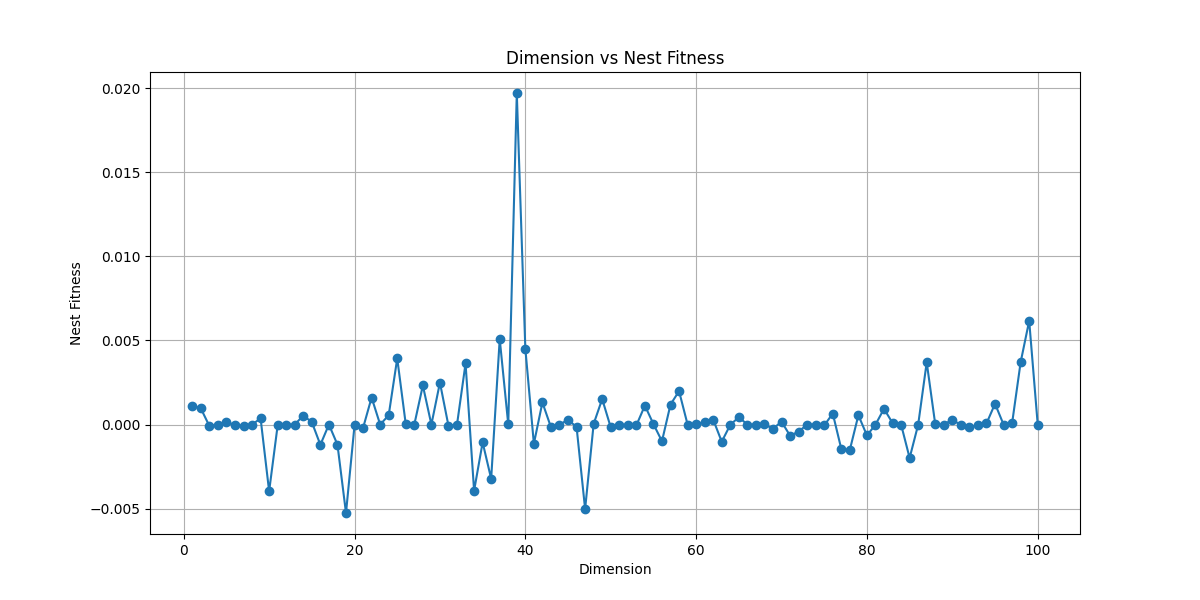
\includegraphics[width=0.8\textwidth]{files/results.png}
    \caption{Cuckoo Search Results}
    \label{fig:results}
\end{figure}

\end{document}
